\newtoggle{bonus} \togglefalse{bonus} % set true to show bonus points in grade table

% setting underlying course name (Grundlagenfach Mathematik, §-Unterricht, ...)
\newcommand{\mycourse}{Grundlagenfach Mathematik}
% name of the class
\newcommand{\myclass}{Klasse 2f}
% set date
\newcommand{\mydate}{23. Juni 2022}

\title{Prüfung
	
\Large{Semesterprüfung}}
\author{Thomas Graf\\
	\mycourse, \myclass}
\date{\mydate}
\maketitle
\thispagestyle{headandfoot}		

\begin{center}
	\fbox{\parbox{140mm}{\centering
			\begin{itemize}
				\item Dauer der Prüfung: $80$ Minuten.
				\item \textbf{Zeigen Sie in jeder Aufgabe unbedingt Ihre Schritte!}
				\item Erlaubte Hilfsmittel:
				\begin{itemize}
				    \item Lineal, Geodreieck, Schreibzeug
				    \item Taschenrechner
				    \item Formelsammlung (Adrian Wetzel)
				\end{itemize}\item In dieser Prüfung werden sämtliche \quotes{Winkel} im Bogenmass angegeben. Verwenden Sie bitte ebenfalls ausschliesslich das Bogenmass.
\item Für $z\in\Cunit$ existiert genau ein $\alpha\in\ico{0}{2\pi}$, so dass $z = \abs{z}e^{i\alpha}$. Diese Zahl $\alpha$  wird \tib{normalisiertes Argument} von $z$ genannt. Wir werden hier stets dieses Argument verwenden.
	\end{itemize}}}
\end{center}
\vspace{10mm}

\begin{center}
	Vorname: \rule{45mm}{0.8pt}\qquad Nachname: \rule{45mm}{0.8pt}
\end{center}
\vspace{20mm}

\begin{center}
	\iftoggle{bonus} {
		\multirowcombinedgradetable{2}[questions]
	} {
		\multirowgradetable{2}[questions]
	}
\end{center}
\vspace{15mm}
\begin{center}
	Note: 
	\vspace{10mm}
	
	\rule{8mm}{1.2pt}
\end{center}
%\thispagestyle{empty}
\clearpage
\lstset{language=Python}

\begin{questions}
\fullwidth{\Large \textbf{Komplexe Zahlen}}
\question[1]
Bestimmen Sie den Betrag $\abs{z}$ der komplexen Zahl $z := -8 - 4i$.
\begin{solution}
\begin{align*}
    \abs{-8-4i} = \sqrt{(-8)^2+(-4)^2} = \sqrt{80} = 4\sqrt{5} \approx 8.944
\end{align*}
\end{solution}


\question[1] Bestimmen Sie sämtliche Lösungen $z\in\C$ der Gleichung
\begin{align*}
    (z - 4)z + 5 = 0.
\end{align*}
\begin{solution}
\begin{align*}
    (z - 4)z + 5 &= 0 \iff \\
    z^2 - 4z + 5 &= 0
\end{align*}
Dies ist eine quadratische Gleichung mit reellen Koeffizienten. Die Diskriminante
\begin{align*}
    D := (-4)^2 - 4\cdot 1\cdot 5 = -4
\end{align*}
ist negativ. Die beiden Lösungen der Gleichung sind somit
\begin{align*}
    z_{1,2} = \frac{4\pm i\sqrt{-D}}{2} = 2 \pm i
\end{align*}
\end{solution}

\question[1] Geben Sie sowohl die Normalform als auch die Polarform der folgenden komplexen Zahl an:
\begin{align*}
    z := \frac{1-i}{2+2i}.
\end{align*}
\begin{solution}
Die Polarform finden wir sofort durch \quotes{Auflösen} des Bruchs (erweitern mit der komplex Konjugierten des Nenners):
\begin{align*}
    \frac{1-i}{2+2i} = -\frac{1}{2}i.
\end{align*}
Die Komplexe Zahl $-i/2$ hat den Betrag $1/2$ und das normalisierte Argument $(3\pi)/2$ und somit die Polarform
\begin{align*}
    -\frac{i}{2} = \frac{e^{\frac{3\pi i}{2}}}{2}.
\end{align*}
\end{solution}

\question
In dieser Aufgaben wollen wir die drei verschiedenen komplexen Lösungen der Gleichung
\begin{align}\label{eq:komplex}
    z^3 = 4+4i
\end{align}
bestimmen.
\begin{parts}
\part[1] Berechnen Sie zuerst den Betrag $r:=\abs{4+4i}$ und das Argument $\gamma :=\Carg{4+4i}$ der komplexen Zahl $4+4i$.
\begin{solution}
\begin{align*}
    r &= \abs{4+4i} = \sqrt{4^2+4^2} = \sqrt{32} = 4\sqrt{2}, \\
    \Carg{4+4i} &= \pi/4
\end{align*}
\end{solution}
\part[1] Wie lauten nun die drei verschiedenen komplexen Lösungen der Gleichung \ref{eq:komplex}.
\droptotalpoints
\begin{solution}
Die drei verschiedenen komplexen Lösungen lauten
\begin{align*}
    z_k = \sqrt[3]{r}e^{\frac{\gamma + 2k\pi}{3}i},
\end{align*}
mit $k\in\lrc{0,1,2}$.
\end{solution}
\end{parts}

\clearpage
\fullwidth{\Large \textbf{Quadratische Funktionen}}
\question[2] Bestimmen Sie die Koordinaten des Scheitelpunkts der quadratischen Funktion 
\begin{align*}
    f(x) = 2x^2 - 4x + 5.
\end{align*}

\begin{solution}
Der Scheitelpunkt $S$ hat die Koordinaten
\begin{align*}
    S = \lr{1,3}.
\end{align*}
\end{solution}

\question[1] Gegeben sind zwei quadratische Funktionen
\begin{align*}
    f(x) &= x^2, \\
    g(x) &= 2x^2+2x-3.
\end{align*}
Bestimmen Sie die Koordinaten der beiden Schnittpunkte dieser Funktionen.
\begin{solution}
Die quadratische Gleichung
\begin{align*}
    x^2 = 2x^2 + 2x - 3
\end{align*}
besitzt die beiden reellen Lösungen $x_1 = -3$ und $x_2 = 1$. Die Koordinaten der Schnittpunkte lauten somit
\begin{align*}
    (-3,9), (1,1).
\end{align*}
\end{solution}

\question[2] Beim kanadischen Grand Prix in der Formel 1 fahren Carlos Sainz und Max Verstappen auf einem Rundkurs. Gerade eben hat Regen eingesetzt und die Rennstrecke ist dadurch nass geworden. Max' Team hat sofort reagiert und seinem Fahrzeug neue Reifen aufgezogen, welche sich für das Fahren auf nasser Fahrbahn gut eignen (\textit{full wets}). Carlos fährt noch immer weiter mit Reifen, welche sich nur für trockenen Untergrund eignen (\textit{slicks}).
\begin{itemize}
    \item Carlos benötigt für jede Rennrunde im Folgenden exakt 7 Sekunden mehr als Max.
    \item Die Teams beobachten, dass Max jeweils in 140 Sekunden genau eine Runde mehr zurücklegt als Carlos in derselben Zeit zurücklegt. Das heisst, Max überrundet Carlos nach 140 Sekunden.
\end{itemize}
Wie lange benötigt Max (in Sekunden) für eine Rennrunde? Wie lange benötigt Carlos?

\noindent
Tipp: Bezeichnen Sie die Rundenzeit von Max mit $A$ und die Rundenzeit von Carlos mit $B$. Stellen Sie zwei Gleichungen für $A$ und $B$ auf. Die eine ist linear, die andere nicht. Lösen Sie die lineare Gleichung nach $A$ auf und setzen Sie $A$ in die zweite Gleichung ein. Dadurch erhalten Sie eine quadratische Gleichung, welche als Unbekannte lediglich $B$ enthält. Lösen Sie diese quadratische Gleichung.

\begin{figure}[H]
    \centering
    \includegraphics[width=0.9\textwidth]{RB18.jpg}
    \caption{Das Formel 1 Fahrzeug \textit{RB18} der Saison 2022 des Teams \textit{Red Bull Racing} mit \textit{blauen Reifen} (full wets) im dritten \textit{freien Training} des grossen Preis von Kanada 2022.}
    \label{fig:RB18}
\end{figure}
\begin{solution}
Die Aufgabenstellung impliziert die beiden Gleichungen
\begin{align*}
    A &= B - 7, \\
    \frac{140}{A} &= \frac{140}{B} + 1.
\end{align*}
Mit dem Tipp erhalten wir die quadratische Gleichung
\begin{align*}
    &\frac{140}{B-7} = \frac{140}{B} + 1 \iff \\
    &B^2 - 7B - 980 = 0,
    \end{align*}
welche die positive Lösung $B = 35$ besitzt. Somit ist die Rundenzeit von Carlos 35 Sekunden und die von Max 28 Sekunden.
\end{solution}

\clearpage
\fullwidth{\Large \textbf{Kombinatorik}}
\question[1]
Es seien $x,y\in\R$. Multiplizieren Sie den Term $(x-y)^5$ vollständig aus. Zeigen Sie Ihre Schritte.
\begin{solution}
Wir verwenden den binomischen Lehrsatz
\begin{align*}
    (a+b)^n  = \sum_{k=0}^n \binom{n}{k}a^{n-k}b^k
\end{align*}
mit der Wahl $a:=x$ und $b:=-y$ und finden sofort
\begin{align*}
    x^5 - 5x^4y + 10x^3y^2 - 10x^2y^3 + 5xy^4 - y^5.
\end{align*}
\end{solution}

\question[1]
Wie viele Wörter der Länge 15 gibt es, welche genau 6 Mal den Buchstaben $a$, genau 4 Mal den Buchstaben $b$ und genau 5 Mal den Buchstaben $c$ enthalten?
\begin{solution}
Es gibt
\begin{align*}
    \binom{15}{6}\binom{9}{4} = \frac{15!}{6!4!5!} = 630630
\end{align*}
Möglichkeiten. (Permutation mit Wiederholung oder Kombination ohne Wiederholung)
\end{solution}

\question[1]
Beim Lotto kreuzt man 6 Zahlen in einem Feld von 45 Zahlen an. Auf wie viele Arten kann man einen Lottozettel ankreuzen, um einen Lotto-5-er zu erzielen? (genau 5 richtige ankreuzen)
\begin{solution}
Stellen Sie sich einen völlig korrekt ausgefüllten Lottozettel (6 richtig angekreuzte Zahlen) vor, der auf dem Tisch liegt. Es gibt $\binom{6}{5}$ Möglichkeiten aus den 6 richtigen Zahlen genau 2 auszuwählen. Für jede dieser Möglichkeiten (Pfadregel) gibt es $\binom{39}{1}$ Möglichkeiten 1 falsche auszuwählen. Insgesamt also
\begin{align*}
     \binom{6}{5}\binom{39}{1} = 234
\end{align*}
Möglichkeiten.
\end{solution}

\question[2] In \cref{fig:gitter} ist ein rechteckiges ($6\times 8$)--Gitter dargestellt, welches aus ($6\times 8$) kleinen Quadraten besteht. Wir betrachten nun ein allgemeines $(n\times m)$--Gitter, mit $n,m\in\Nunit$. In jedem Schritt können Sie entweder genau eine Kantenlänge eines kleinen Quadrats nach unten oder nach rechts gehen. Sie beginnen Ihren Pfad bei \textit{Start}. Wie viele verschiedene Pfade von \textit{Start} nach \textit{Ziel} sind in einem $(n\times m)$--Gitter möglich? In \cref{fig:gitter} ist ein möglicher Pfad in einem $(6\times 8)$--Gitter \textcolor{red}{rot} eingezeichnet.
\begin{figure}[H]
    \centering
    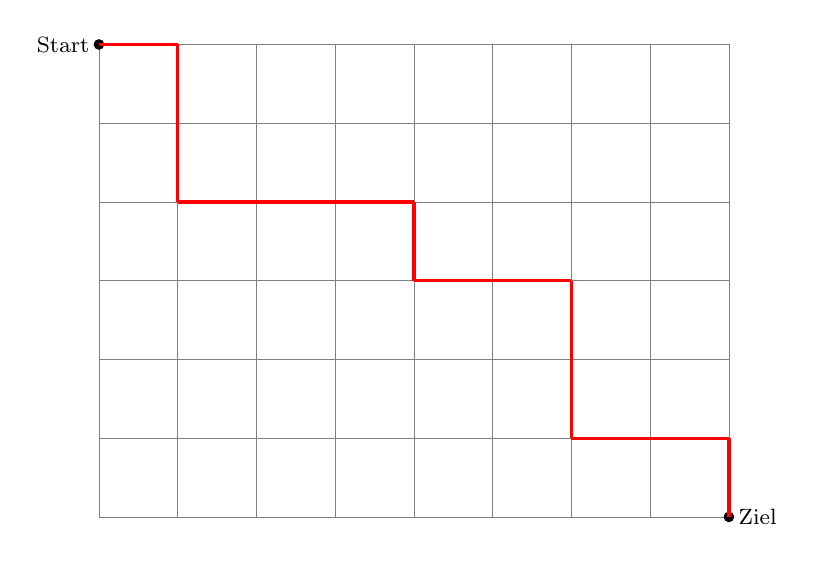
\begin{tikzpicture}
    \draw[step=1cm,gray,very thin] (-2,-2) grid (6,4);
    \draw [fill] (-2,4) circle [radius=.06] node[left] {{\footnotesize Start}};
    \draw [fill] (6,-2) circle [radius=.06] node[right] {{\footnotesize Ziel}};
    \draw [very thick, red] (-2,4) -- (-1,4);
    \draw [very thick, red] (-1,4) -- (-1,2);
    \draw [very thick, red] (-1,2) -- (2,2);
    \draw [very thick, red] (2,2) -- (2,1);
    \draw [very thick, red] (2,1) -- (4,1);
    \draw [very thick, red] (4,1) -- (4,-1);
    \draw [very thick, red] (4,-1) -- (6,-1);
    \draw [very thick, red] (6,-1) -- (6,-2);
    \end{tikzpicture}
    \caption{Anzahl der Pfade in einem rechteckigen Gitter.}
    \label{fig:gitter}
\end{figure}
\begin{solution}
Jeder gültige Pfad lässt sich durch genau ein Wort der Länge $n+m$ repräsentieren, welches genau $n$ mal den Buchstaben $u$ (\textbf{unten}) enthält und genau $m$ mal den Buchstaben $r$ (\textbf{r}echts). Der rote Pfad in \cref{fig:gitter} wird also durch das Wort
\begin{align*}
    ruurrrurruurru
\end{align*}
dargestellt. Die Anzahl dieser Wörter ist gegeben durch
\begin{align*}
    \frac{(n+m)!}{n!m!}.
\end{align*}
(Permutation mit Wiederholung)
\end{solution}
\end{questions}